\documentclass[letterpaper,openany,oneside,twocolumn]{book}

\usepackage[justified]{dnd}
\usepackage{ifthen}

\usepackage{dndtemplate}
\usepackage{bookmark}

\setlength\oddsidemargin{\dimexpr(\paperwidth-\textwidth)/2 - 1in\relax}
\setlength\evensidemargin{\oddsidemargin}

% Headline
\CharacterName{Hilmar Frodeveld}

% adds only main class and total level to prevent overflow
\Class{Cleric 5}
\Background{Gambler}
\PlayerName{PJBrs}
\Race{Lightfoot Halfling}
\Alignment{Neutral good}
\XP{Milestone}

% Ability scores
\StrengthScore{10}
\DexterityScore{15}
\ConstitutionScore{10}
\IntelligenceScore{12}
\WisdomScore{17}
\CharismaScore{14}

% Ability modifiers
\StrengthModifier{0}
\DexterityModifier{2}
\ConstitutionModifier{0}
\IntelligenceModifier{1}
\WisdomModifier{2}
\CharismaModifier{2}

% Saving Throws
\StrengthSavingThrowModifier{0}
\DexteritySavingThrowModifier{2}
\ConstitutionSavingThrowModifier{0}
\IntelligenceSavingThrowModifier{1}
\WisdomSavingThrowModifier{4}
\CharismaSavingThrowModifier{4}

\AcrobaticsSkillModifier{2}
\AnimalHandlingSkillModifier{2}
\ArcanaSkillModifier{1}
\AthleticsSkillModifier{0}
\DeceptionSkillModifier{2}
\HistorySkillModifier{1}
\InsightSkillModifier{4}
\IntimidationSkillModifier{2}
\InvestigationSkillModifier{1}
\MedicineSkillModifier{2}
\NatureSkillModifier{1}
\PerceptionSkillModifier{4}
\PerformanceSkillModifier{2}
\PersuasionSkillModifier{4}
\ReligionSkillModifier{3}
\SleightOfHandSkillModifier{2}
\StealthSkillModifier{2}
\SurvivalSkillModifier{2}

% Proficiencies
\SetStrengthProficiency{0}
\SetDexterityProficiency{0}
\SetConstitutionProficiency{0}
\SetIntelligenceProficiency{0}
\SetWisdomProficiency{1}
\SetCharismaProficiency{1}

\SetAcrobaticsProficiency{0}
\SetAnimalHandlingProficiency{0}
\SetArcanaProficiency{0}
\SetAthleticsProficiency{0}
\SetDeceptionProficiency{0}
\SetHistoryProficiency{0}
\SetInsightProficiency{1}
\SetIntimidationProficiency{0}
\SetInvestigationProficiency{0}
\SetMedicineProficiency{0}
\SetNatureProficiency{0}
\SetPerceptionProficiency{1}
\SetPerformanceProficiency{0}
\SetPersuasionProficiency{1}
\SetReligionProficiency{1}
\SetSleightOfHandProficiency{0}
\SetStealthProficiency{0}
\SetSurvivalProficiency{0}

\Inspiration{}
\Proficiency{2}
\Perception{14}

\ArmorClass{17}
\Initiative{2}
\Speed{25}
\MaxHitPoints{21}


\MaxHitDice{2d8}
\CurrentHitDice{}

\CP{}
\SP{}
\GP{}
\EP{}
\PP{}


\AddWeapon{Sling}{+4}{1d4+2/b}

\AddWeapon{Mace}{+2}{1d6/b}

\AddWeapon{Unarmed}{+2}{1/b}


\AttacksAdditional{\textbf{Armor}: Chain Shirt \\
\textbf{Shield}: Shield \\
\textbf{Sacred Flame}: sv. 12 (dex), dmg 1d8/r \\
\textbf{Guiding Bolt}: att. +4, dmg 4d6/r \\
\textbf{Holy Symbol}: a coin depicting the push and pull of luck and fate
}

\OtherProficienciesLanguages{\textbf{Languages:} Common, Halfling. \\
\textbf{Weapons}: Simple Weapons. \\
\textbf{Armor}: Light Armor, Medium Armor, Shields. \\
\textbf{Other}: Flute, Playing Card Set. \\}

\Equipment{
Sling, 20 Sling Bullets, Mace, Backpack, Bedroll, Mess Kit, Tinderbox, 10 Torches,
10 Days of Rations, Waterskin, 50 Feet of Hempen Rope, Pouch, Deck of Cards
\\ \footnotesize{
\textbf{Weight:} 96 lb \textbf{Capacity:} 150 lb
}}

\PersonalityTraits{Daring. I like to make people take a chance. And I like to put them off balance.}

\Ideals{Creativity. The world is in need of new ideas and bold action. (Chaotic.)}

\Bonds{I'm torn! Secretly, I'd like to go home. But my religious commitments have led me abroad...}

\Flaws{I have trouble keeping my true feelings hidden. My sharp tongue lands me in trouble.}

\FeaturesTraits{
\textbf{Features} \\
Blessing of the Trickster \\
Channel Divinity (1x/SR) \\
Channel Divinity: Turn Undead \\
Channel Divinity: Invoke Duplicity \\
Lucky \\
Brave \\
Halfling Nimbleness \\
Naturally Stealthy \\
Never Tell Me the Odds
}


% Appearance

\Age{21}
\Height{2'9}
\Weight{39lbs}
\Eyes{Green}
\Skin{Tan}
\Hair{Brown}

% background

\CharacterAppearance{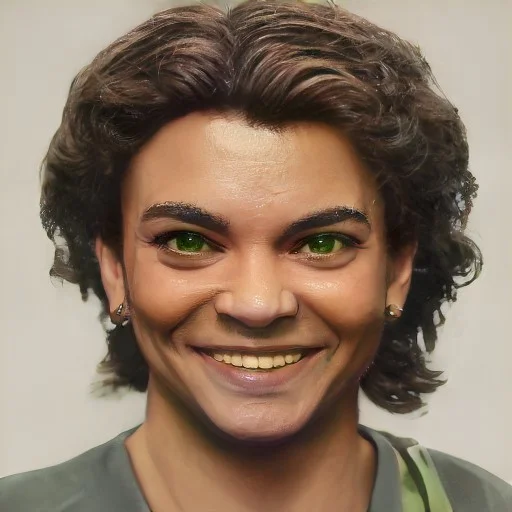
\includegraphics[width=5.75cm]{characters/images/hilmar.jpeg}


}
\AdditionalFeaturesAndTraits{I was the second son in our family. And as family tradition dictated, I was to dedicate my life to religion. Our local cleric took up
my training. We were a class of three. And pretty soon, it was clear that the clerical life was not for me. But it wasn't that
supernatural presences were completely outside my grasp. That is, some of the religious teachings strangely escaped my grasp, but others
I could make happen quite well. Healing was no problem. One thing became clearer and clearer to me - my religious experience was very
different from the the one of my peers.

And in class, I kept feeling my mind drift. And during my offtime, I found myself playing at cards and dice. I played the flute in the
tavern. Could almost have been a bard. I made bets with my friends during the yearly festival, we bet on sports, dogs, even children
playing. Everywhere, I found myself drawn to wherever chance could make a big difference. And when finally I noticed how may little
games co-occurred with that supernatural presence, I found my calling. I said my goodbyes, became my own cleric, and left town on
my first big bet.
}

\Characterbackground{I've always been fascinated with chance. The first time I had dared my baby sister to climb a tree near our home. As she climbed higher, I felt the hairs on my feet
rise. And just when my neck started to tingle, my sister lost her grip, fell down, and landed head first on a rock. Unscathed.

The second time, I had postponed my chores for the better part of the day, and my dad had begun to lose his temper. As
he crossed the room, I felt that same tingle. He bumped his toe, tumbled forward, landed on a pillow, and broke his neck. Dead.
That day, I learned not to tempt the powers of fate and luck, for the Lady may pull, but the Lord might push. And that's how I
became a religious man.

I more and more felt the Lady's pull. Soon after, I began to hold bets, to dare people to test their luck. I always carried my dice with
me, and at our festival, I encouraged people to make bets and take chances. Last year, I made a bet ad cast the dice myself:
A week of revelry for the Lady's pull, or a week away from home on my own for the Lord's push.
I lost that one, and now it has been much longer than a week since I left home...
}

\Treasure{
}

\AlliesAndOrganizations{
}

\OrganizationName{\centering{Clan Frodeveld}
}


%Magic
\SpellcastingClass{Cleric 5}
\SpellcastingAbility{WIS}
\SpellSaveDC{14}
\SpellAttackBonus{+6}

\FirstLevelSpellSlotsTotal{4}
\SecondLevelSpellSlotsTotal{3}
\ThirdLevelSpellSlotsTotal{2}


\begin{document}
\newgeometry{left=0cm,right=0cm,top=0cm,bottom=0cm}
\onecolumn


% CHARACTER PAGE
\pdfbookmark[0]{Character Sheet}{Character Sheet}
\rendercharactersheet

% BACKSTORY PAGE
\pdfbookmark[0]{Background Sheet}{Background Sheet}
\renderbackgroundsheet

% SPELLCASTING PAGE
\pdfbookmark[0]{Spellcasting Sheet}{Spellcasting Sheet}
\CantripSlotA{Fast Friends}
\CantripSlotB{Guidance (V/S/C)}
\CantripSlotC{Incite Greed}
\CantripSlotD{Motivational Speech}
\CantripSlotE{Sacred Flame (V/S)}
\CantripSlotF{Spirit Shroud}
\CantripSlotG{Thaumaturgy (V)}
\FirstLevelSpellSlotA{Bane (V/S/M/C)}
\FirstLevelSpellSlotB{Bless (V/S/M/C)}
\FirstLevelSpellSlotBPrepared{True}
\FirstLevelSpellSlotC{Ceremony (V/S/M/R/\$)}
\FirstLevelSpellSlotD{Charm Person (V/S)}
\FirstLevelSpellSlotDPrepared{True}
\FirstLevelSpellSlotE{Command (V)}
\FirstLevelSpellSlotF{Create Or Destroy Water (V/S/M)}
\FirstLevelSpellSlotG{Cure Wounds (V/S)}
\FirstLevelSpellSlotGPrepared{True}
\FirstLevelSpellSlotH{Detect Evil And Good (V/S/C)}
\FirstLevelSpellSlotI{Detect Magic (V/S/R/C)}
\FirstLevelSpellSlotIPrepared{True}
\FirstLevelSpellSlotJ{Detect Poison And Disease (V/S/M/C)}
\FirstLevelSpellSlotK{Disguise Self (V/S)}
\FirstLevelSpellSlotKPrepared{True}
\FirstLevelSpellSlotL{Guiding Bolt (V/S)}
\FirstLevelSpellSlotLPrepared{True}
\FirstLevelSpellSlotM{Guiding Hand (V/S/R/C)}
\FirstLevelSpellSlotN{Healing Word (V)}
\FirstLevelSpellSlotO{Inflict Wounds (V/S)}
\FirstLevelSpellSlotP{Protection From Evil And Good (V/S/M/C)}
\FirstLevelSpellSlotQ{Purify Food And Drink (V/S/R)}
\FirstLevelSpellSlotR{Sanctuary (V/S/M)}
\FirstLevelSpellSlotS{Shield Of Faith (V/S/M/C)}

\SecondLevelSpellSlotA{Aid (V/S/M)}
\SecondLevelSpellSlotB{Augury (V/S/M/R/\$)}
\SecondLevelSpellSlotC{Blindness/Deafness (V)}
\SecondLevelSpellSlotD{Calm Emotions (V/S/C)}
\SecondLevelSpellSlotDPrepared{True}
\SecondLevelSpellSlotE{Continual Flame (V/S/M/\$)}
\SecondLevelSpellSlotF{Enhance Ability (V/S/M/C)}
\SecondLevelSpellSlotG{Find Traps (V/S)}
\SecondLevelSpellSlotH{Gentle Repose (V/S/M/R)}
\SecondLevelSpellSlotI{Hold Person (V/S/M/C)}
\SecondLevelSpellSlotJ{Lesser Restoration (V/S)}
\SecondLevelSpellSlotK{Locate Object (V/S/M/C)}
\SecondLevelSpellSlotL{Mirror Image (V/S)}
\SecondLevelSpellSlotLPrepared{True}
\SecondLevelSpellSlotM{Pass Without Trace (V/S/M/C)}
\SecondLevelSpellSlotMPrepared{True}
\SecondLevelSpellSlotN{Prayer Of Healing (V)}
\SecondLevelSpellSlotO{Protection From Poison (V/S)}
\SecondLevelSpellSlotP{Silence (V/S/R/C)}
\SecondLevelSpellSlotQ{Spiritual Weapon (V/S)}
\SecondLevelSpellSlotQPrepared{True}
\SecondLevelSpellSlotR{Warding Bond (V/S/M/\$)}
\SecondLevelSpellSlotS{Zone Of Truth (V/S)}

\ThirdLevelSpellSlotA{Animate Dead (V/S/M)}
\ThirdLevelSpellSlotB{Aura Of Vitality (V/C)}
\ThirdLevelSpellSlotBPrepared{True}
\ThirdLevelSpellSlotC{Beacon Of Hope (V/S/C)}
\ThirdLevelSpellSlotD{Bestow Curse (V/S/C)}
\ThirdLevelSpellSlotE{Blink (V/S)}
\ThirdLevelSpellSlotEPrepared{True}
\ThirdLevelSpellSlotF{Clairvoyance (V/S/M/C/\$)}
\ThirdLevelSpellSlotG{Create Food And Water (V/S)}
\ThirdLevelSpellSlotH{Daylight (V/S)}
\ThirdLevelSpellSlotI{Dispel Magic (V/S)}
\ThirdLevelSpellSlotIPrepared{True}
\ThirdLevelSpellSlotJ{Feign Death (V/S/M/R)}
\ThirdLevelSpellSlotK{Glyph Of Warding (V/S/M/\$)}
\ThirdLevelSpellSlotL{Life Transference (V/S)}
\ThirdLevelSpellSlotM{Magic Circle (V/S/M/\$)}
\ThirdLevelSpellSlotN{Mass Healing Word (V)}
\ThirdLevelSpellSlotO{Meld Into Stone (V/S/R)}
\ThirdLevelSpellSlotP{Protection From Energy (V/S/C)}
\ThirdLevelSpellSlotQ{Remove Curse (V/S)}
\ThirdLevelSpellSlotR{Revivify (V/S/M/\$)}
\ThirdLevelSpellSlotS{Sending (V/S/M)}

\renderhalfspellsheet

\CantripSlotA{}
\CantripSlotB{}
\CantripSlotC{}
\CantripSlotD{}
\CantripSlotE{}
\CantripSlotF{}
\CantripSlotG{}

\FirstLevelSpellSlotA{}
\FirstLevelSpellSlotB{}
\FirstLevelSpellSlotBPrepared{False}
\FirstLevelSpellSlotC{}
\FirstLevelSpellSlotD{}
\FirstLevelSpellSlotDPrepared{False}
\FirstLevelSpellSlotE{}
\FirstLevelSpellSlotF{}
\FirstLevelSpellSlotG{}
\FirstLevelSpellSlotGPrepared{False}
\FirstLevelSpellSlotH{}
\FirstLevelSpellSlotI{}
\FirstLevelSpellSlotIPrepared{False}
\FirstLevelSpellSlotJ{}
\FirstLevelSpellSlotK{}
\FirstLevelSpellSlotKPrepared{False}
\FirstLevelSpellSlotL{}
\FirstLevelSpellSlotLPrepared{False}
\FirstLevelSpellSlotM{}
\FirstLevelSpellSlotN{}
\FirstLevelSpellSlotO{}
\FirstLevelSpellSlotP{}
\FirstLevelSpellSlotQ{}
\FirstLevelSpellSlotS{}
\FirstLevelSpellSlotR{}

\SecondLevelSpellSlotA{}
\SecondLevelSpellSlotB{}
\SecondLevelSpellSlotC{}
\SecondLevelSpellSlotD{}
\SecondLevelSpellSlotDPrepared{False}
\SecondLevelSpellSlotE{}
\SecondLevelSpellSlotF{}
\SecondLevelSpellSlotG{}
\SecondLevelSpellSlotH{}
\SecondLevelSpellSlotI{}
\SecondLevelSpellSlotJ{}
\SecondLevelSpellSlotK{}
\SecondLevelSpellSlotL{}
\SecondLevelSpellSlotLPrepared{False}
\SecondLevelSpellSlotM{}
\SecondLevelSpellSlotMPrepared{False}
\SecondLevelSpellSlotN{}
\SecondLevelSpellSlotO{}
\SecondLevelSpellSlotP{}
\SecondLevelSpellSlotQ{}
\SecondLevelSpellSlotQPrepared{False}
\SecondLevelSpellSlotR{}
\SecondLevelSpellSlotS{}

\ThirdLevelSpellSlotA{--- Overflow ---}
\ThirdLevelSpellSlotB{Speak With Dead (V/S/M)}
\ThirdLevelSpellSlotBPrepared{False}
\ThirdLevelSpellSlotC{Spirit Guardians (V/S/M/C)}
\ThirdLevelSpellSlotD{Tongues (V/M)}
\ThirdLevelSpellSlotE{Water Walk (V/S/M/R)}
\ThirdLevelSpellSlotEPrepared{False}
\ThirdLevelSpellSlotF{}
\ThirdLevelSpellSlotG{}
\ThirdLevelSpellSlotH{}
\ThirdLevelSpellSlotI{}
\ThirdLevelSpellSlotIPrepared{False}
\ThirdLevelSpellSlotJ{}
\ThirdLevelSpellSlotK{}
\ThirdLevelSpellSlotL{}
\ThirdLevelSpellSlotM{}
\ThirdLevelSpellSlotN{}
\ThirdLevelSpellSlotO{}
\ThirdLevelSpellSlotP{}
\ThirdLevelSpellSlotQ{}
\ThirdLevelSpellSlotR{}
\ThirdLevelSpellSlotS{}

\renderhalfspellsheet

\end{document}
